\subsubsection{Диаграммы последовательностей}

При программировании некоторых функций проекта, бывает полезно иметь план взаимодействия объектов, это позволяет следовать каждому пункту, заранее разработанного, плана, не задумываясь как все должно работать вместе, что позволяет избежать многих ошибок и, как следствие, спасает разработчика от постоянной переработки логики. Для составления таких планов взаимодействия существуют диаграммы взаимодействия.

Диаграмма взаимодействия – диаграмма, которая описывает взаимодействие определённых объектов в различных ситуациях и условиях их поведения. В языке UML существует несколько типов диаграмм взаимодействия, самым популярным из них являются диаграммы последовательностей.

Диаграмма последовательности (sequence diagram) – диаграмма, которая на временной оси показывает жизненный цикл какого-либо определённого объекта (создание, уничтожения или деятельность некоторой сущности) для некого набора объектов.

Основными элементами диаграммы последовательности являются:
\begin{enumerate}
	\item[1] Объекты. На диаграмме изображаются как прямоугольниками с названиями объектов.
	\item[2] Линии жизни. На диаграмме изображаются пунктирными, вертикальными линиями, отражают течение времени.
	\item[3] Прямоугольники, которые отражают деятельность объекта или исполнение им определенной функции. На диаграмме размещаются на пунктирной линии жизни.
	\item[4] Стрелки, показывающие обмен сигналами или сообщениями между объектами.
\end{enumerate}

Одна из основных возможностей пользователей приложения – прикрепление отсканированных документов. Этот процесс взаимодействует с браузерным приложением СЭД, сканером а так же сервером, на который будут отправляться отсканированные документы.

Рассмотрим диаграмму последовательности для процесса прикрепления файла (рисунок 5.6).

\begin{figure}[h!]
	\centering
	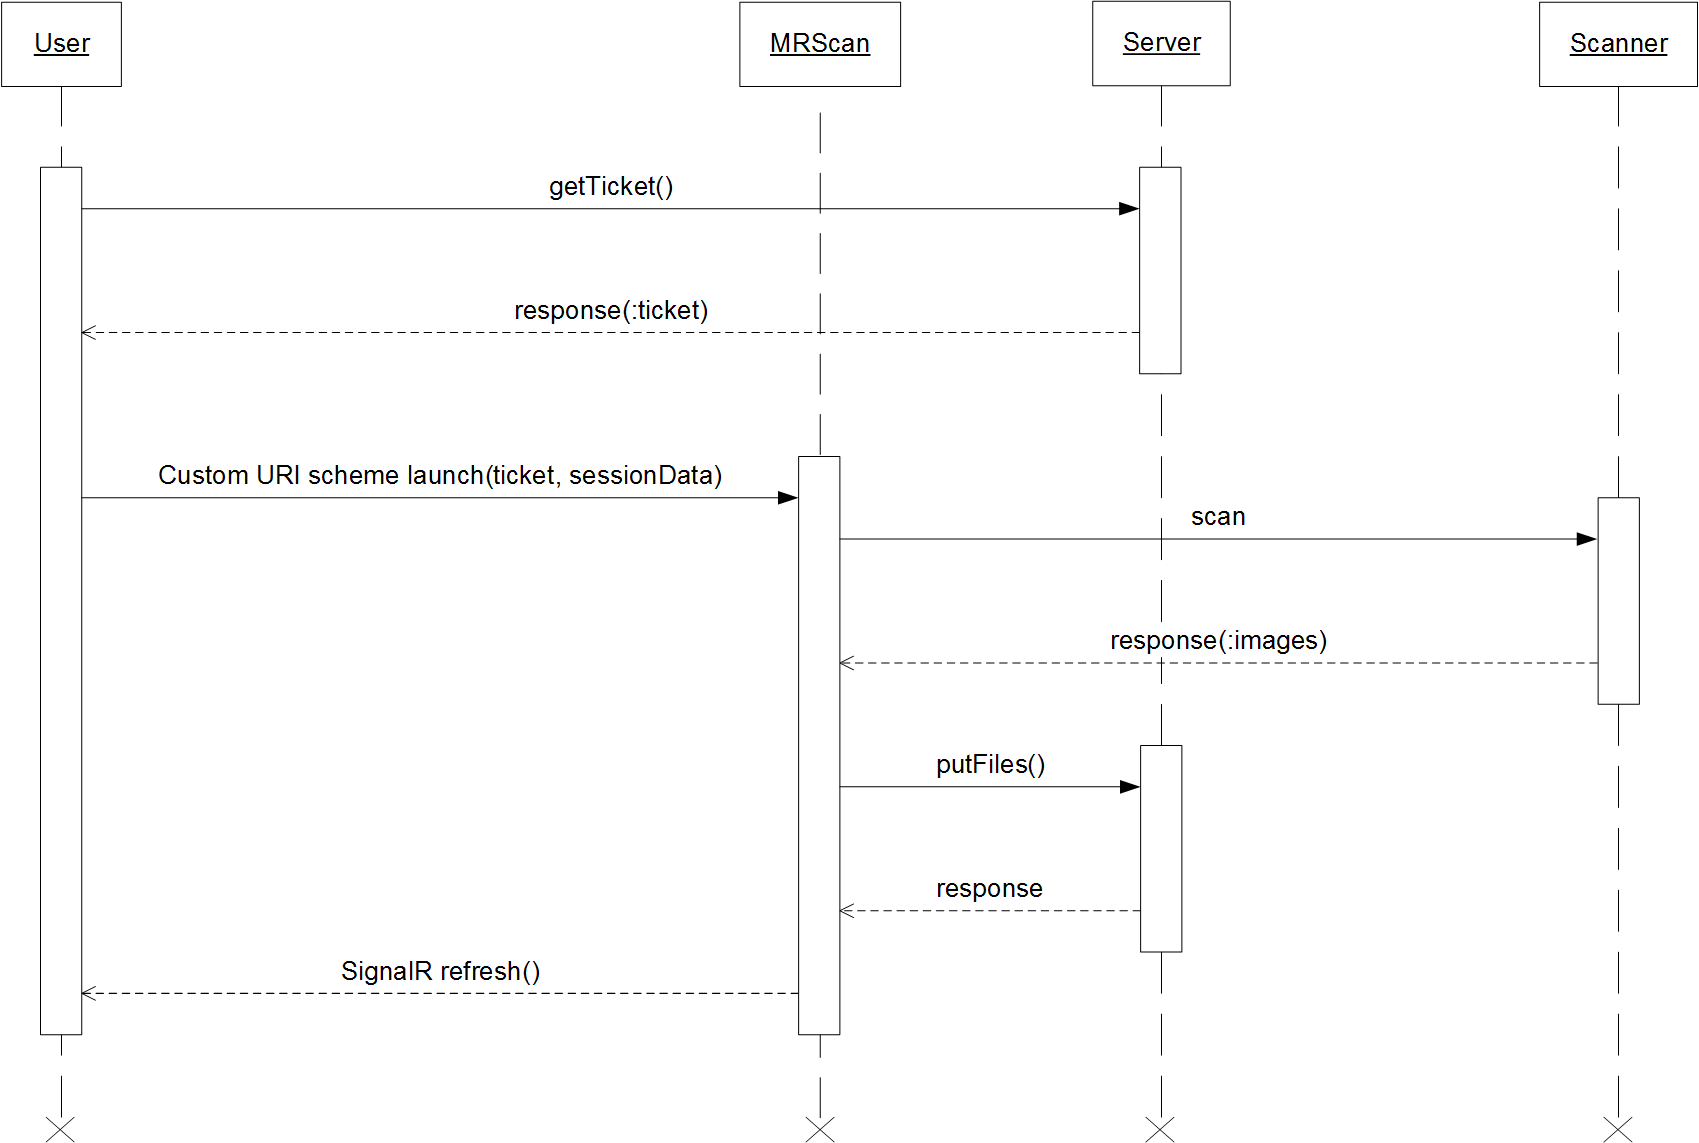
\includegraphics[scale=0.38]{pd3_sequence_general_withoutHeader.png}
	\caption{Диаграмма основной последовательности прикрепления файлов}
\end{figure}

Запуск процесса инициируется пользователем по нажатию на кнопку «Сканировать» в веб-приложении. По нажатию на данную кнопку, требуется запросить создание тикета, который будет использован в дальнейшем для прикрепления файлов. Тикет создается на серверной части. Сервер возвращает идентификатор тикета и время его создания. Далее через Custom URI запускается главное приложение (MRScan), так же через Custom URI передается вся необходимая информация. После запуска приложения, пользователь может начинать сканирование документов. Для этого действия требуется нажать на кнопку «Сканировать», на этот раз в MRScan. Нажатие на кнопку запускает сканирование, отсканированные странички начнут добавляться в список по мере сканирования. Когда сканирование завершится у пользователя есть возможность внести изменения в порядок следования страниц, а так же повернуть страницы, которые могли быть вставлены неверной стороной. Если некоторые страницы были ошибочно переданы сканеру, либо сканирование было осуществлено некачественно, есть возможность удалить ненужные страницы. Когда пользователь определился с контентом будущего докумкнта, он нажимает кнопку «Прикрепить», это запускает функцию putFiles(), в которой на основе ранее полученных данных через Custom URI, создается тикет и на основе тикета, вызывается метод WCF сервиса, который отправляет прикрепляемый файл на сервер окуда он попадает в базу данных. После того как файл успешно прикрепился, MRScan отправляет через SignalR сообщение веб-приложению, которое обновляет страничку и сразу отображает прикрепленный файл. 

\begin{figure}[h!]
	\centering
	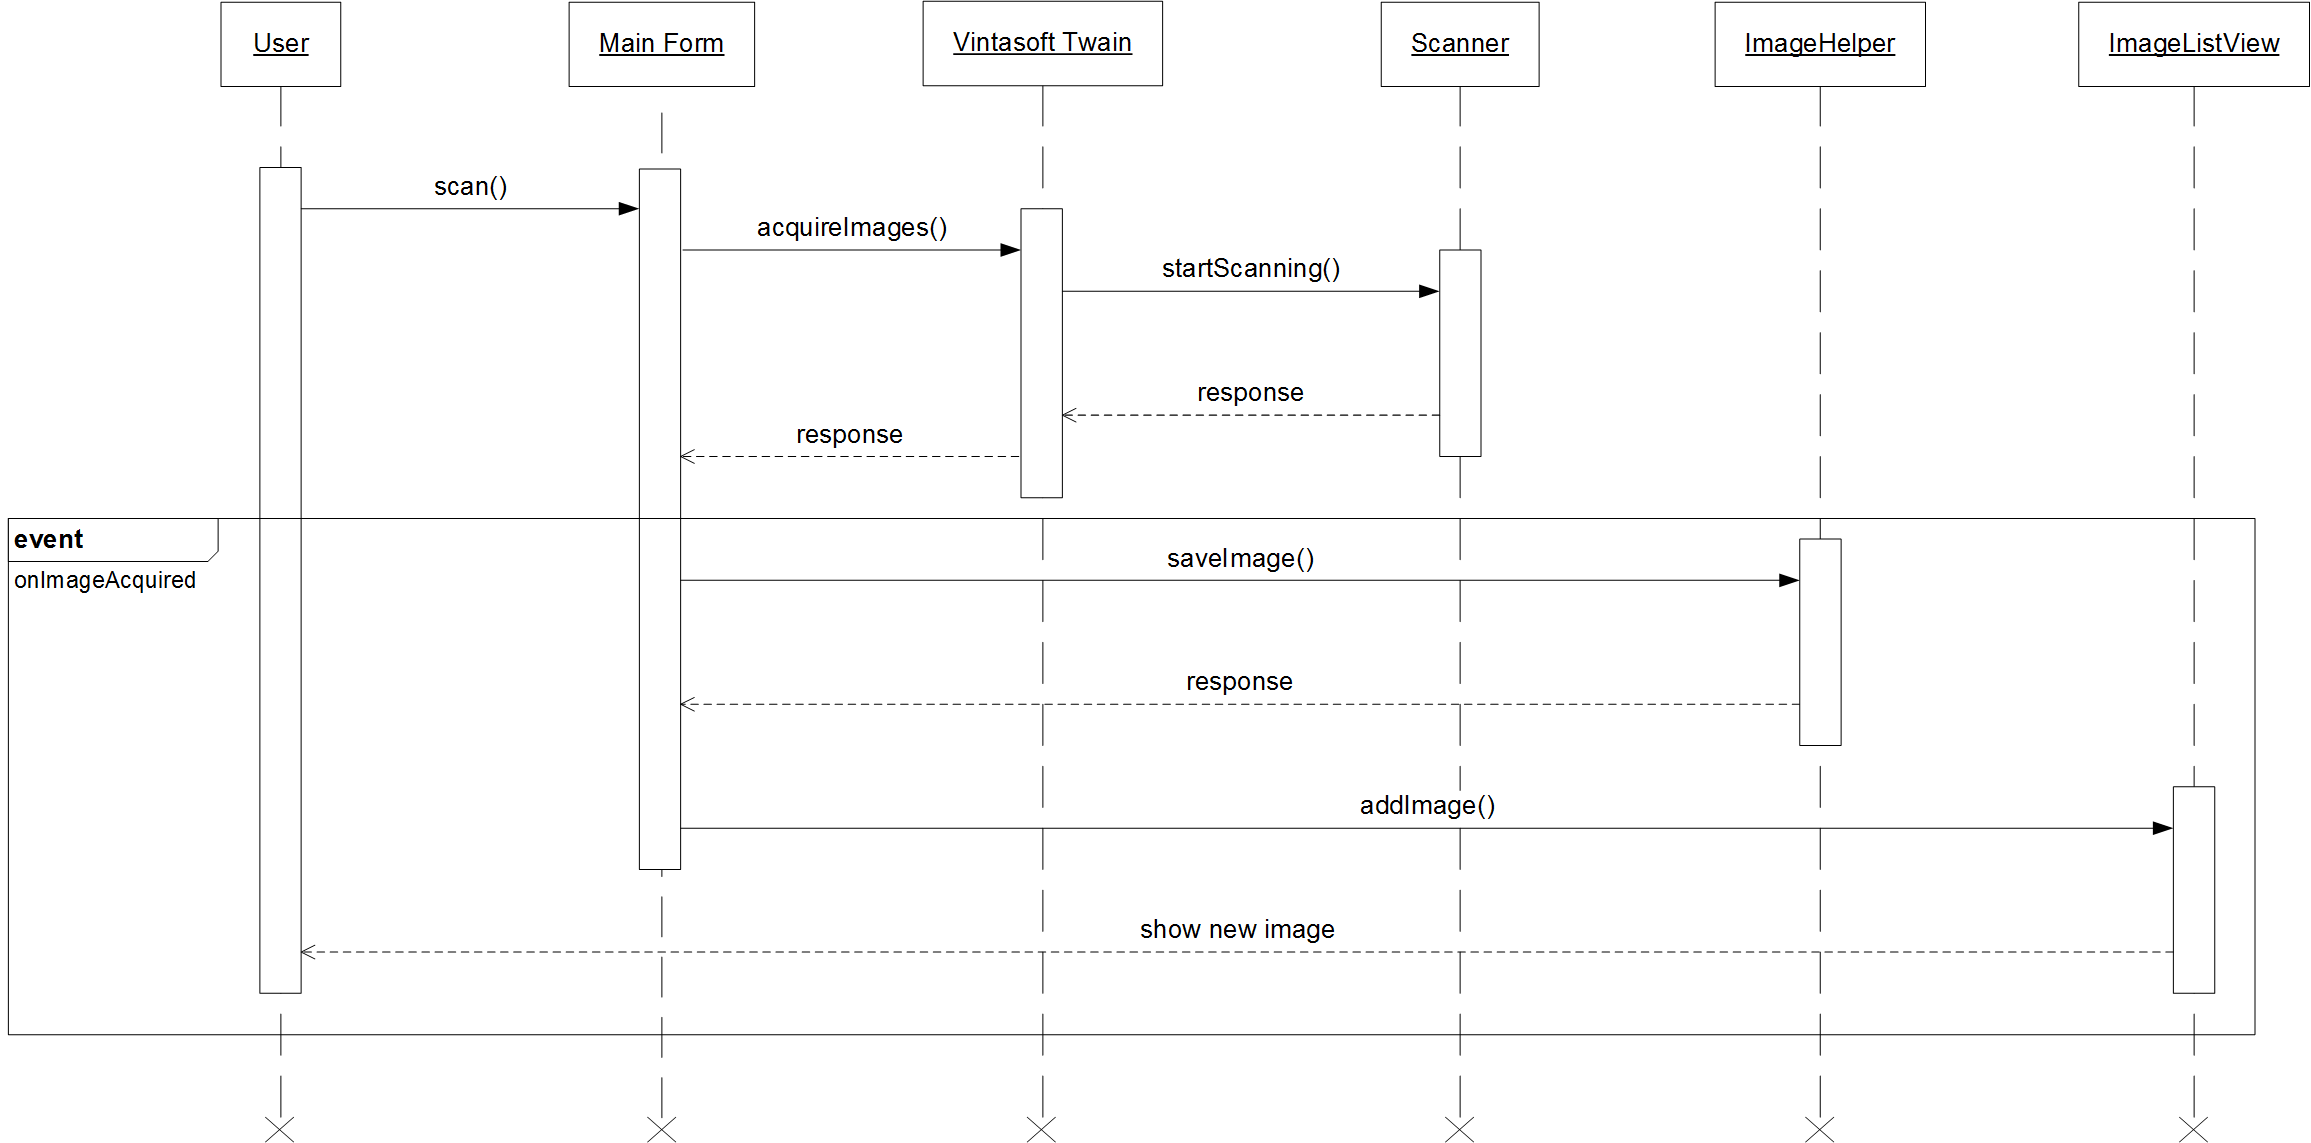
\includegraphics[scale=0.3]{pd4_sequence_withoutHeader.png}
	\caption{Диаграмма последовательности сканирования}
\end{figure}